% !TeX root = ../defense.tex

\section{Topological Data Analysis}
\frame{\sectionpage}

\begin{frame}{What is topology?}
\begin{columns}
\begin{column}{0.6\linewidth}
\uncover<+->{
	\centering
	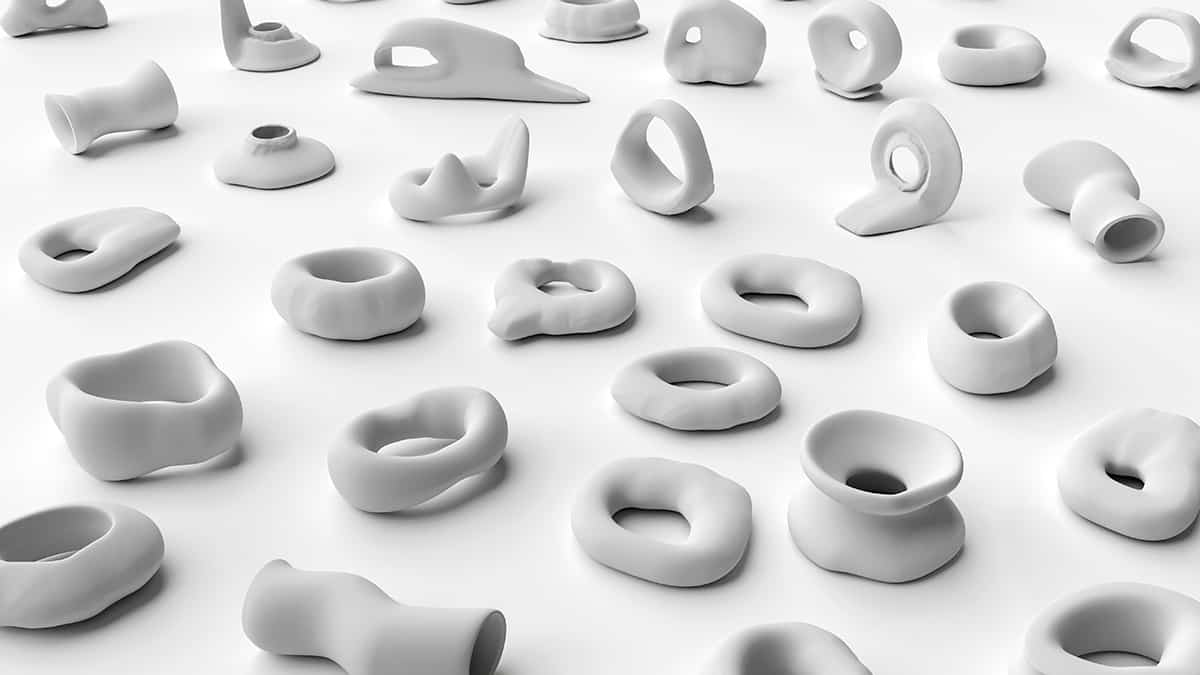
\includegraphics[width=\linewidth]{img/Topological_homeomorphism}\\
	\textcolor{gray}{\fontsize{6.5}{10}\selectfont Image credit: \href{https://physicsworld.com/a/its-topology-naturally/}{Physics world}}
}
\end{column}
\begin{column}{0.4\linewidth}
\uncover<+->{Topology:}
\begin{itemize}[<+->]
	\item The study of holes
	\item Rubber-sheet geometry\\~\\
\end{itemize}
\uncover<+->{Branches of topology:}
\begin{itemize}[<+->]
	\item General Topology or Point Set Topology
	\item Combinatorial Topology
	\item Differential Topology
	\item \boxed{Algebraic Topology}
\end{itemize}
\end{column}
\end{columns}
\end{frame}

\begin{frame}{Homeomorphism}
\begin{columns}
\begin{column}{0.6\linewidth}
\uncover<+->{
	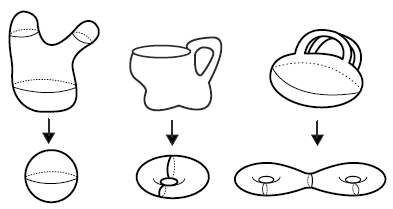
\includegraphics[width=0.6\linewidth]{img/surfaces}\\
	\textcolor{gray}{\fontsize{6.5}{10}\selectfont Image credit: \href{https://uregina.ca/~franklam/Math441_F2019.html}{Annenberg Learner}}\\~\\
}
$\uncover<3->{\beta_k(\psi)} \uncover<4->{= \dim (H_k(\psi))}$\\~\\
\uncover<5->{
	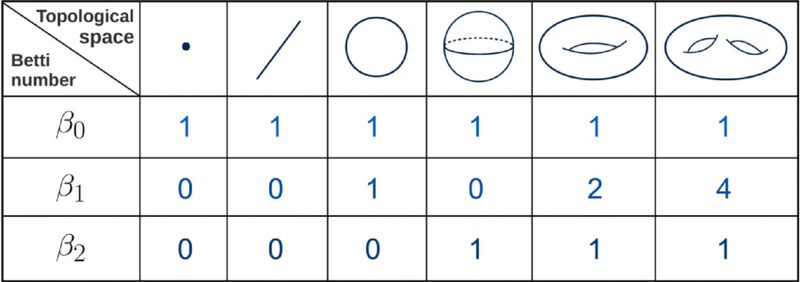
\includegraphics[width=.9\linewidth]{img/betti_numbers}\\
	\textcolor{gray}{\fontsize{6.5}{10}\selectfont Image credit: \href{https://journals.aps.org/pre/abstract/10.1103/PhysRevE.104.034116}{Masoomy, et al.}}
}
\end{column}
\begin{column}{0.4\linewidth}
\uncover<2->{
	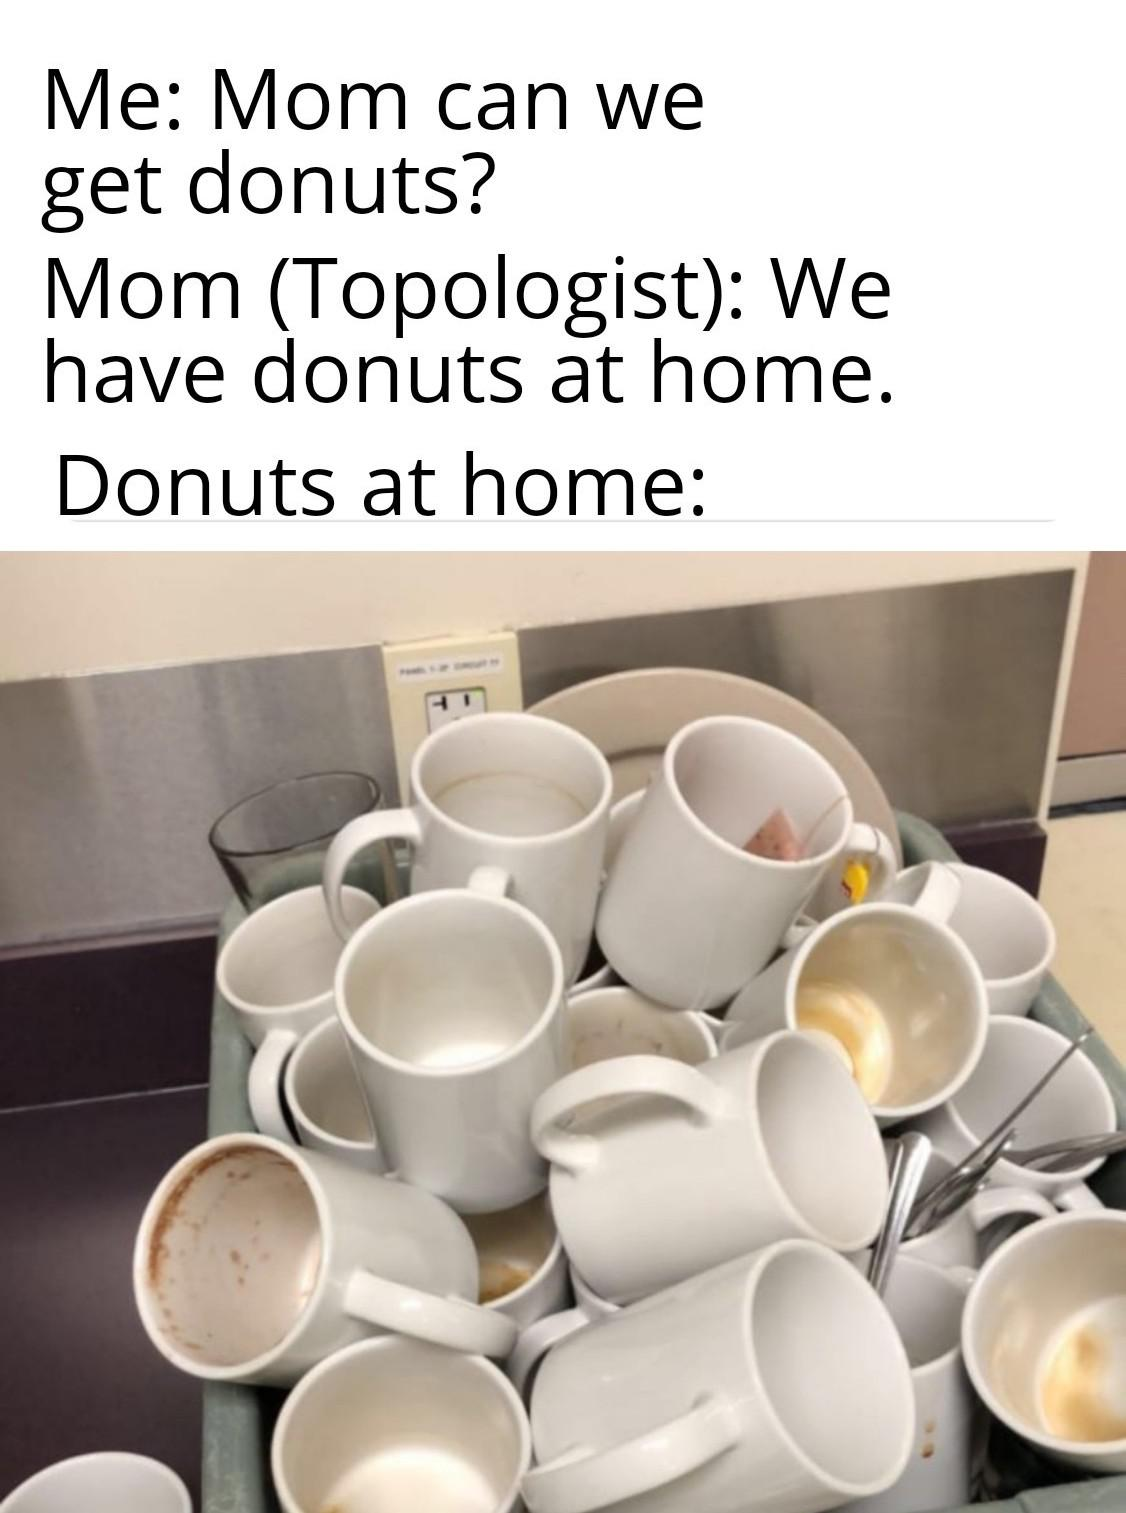
\includegraphics[width=\linewidth]{img/meme}
	\textcolor{gray}{\fontsize{6.5}{10}\selectfont Image source: \href{https://www.reddit.com/r/mathmemes/comments/eilb2c/donuts_at_home/}{Reddit}}
}
\end{column}
\end{columns}
\end{frame}

\begin{frame}{Topology of time series}
\begin{columns}
\begin{column}{0.6\linewidth}
\centering
\uncover<+->{
	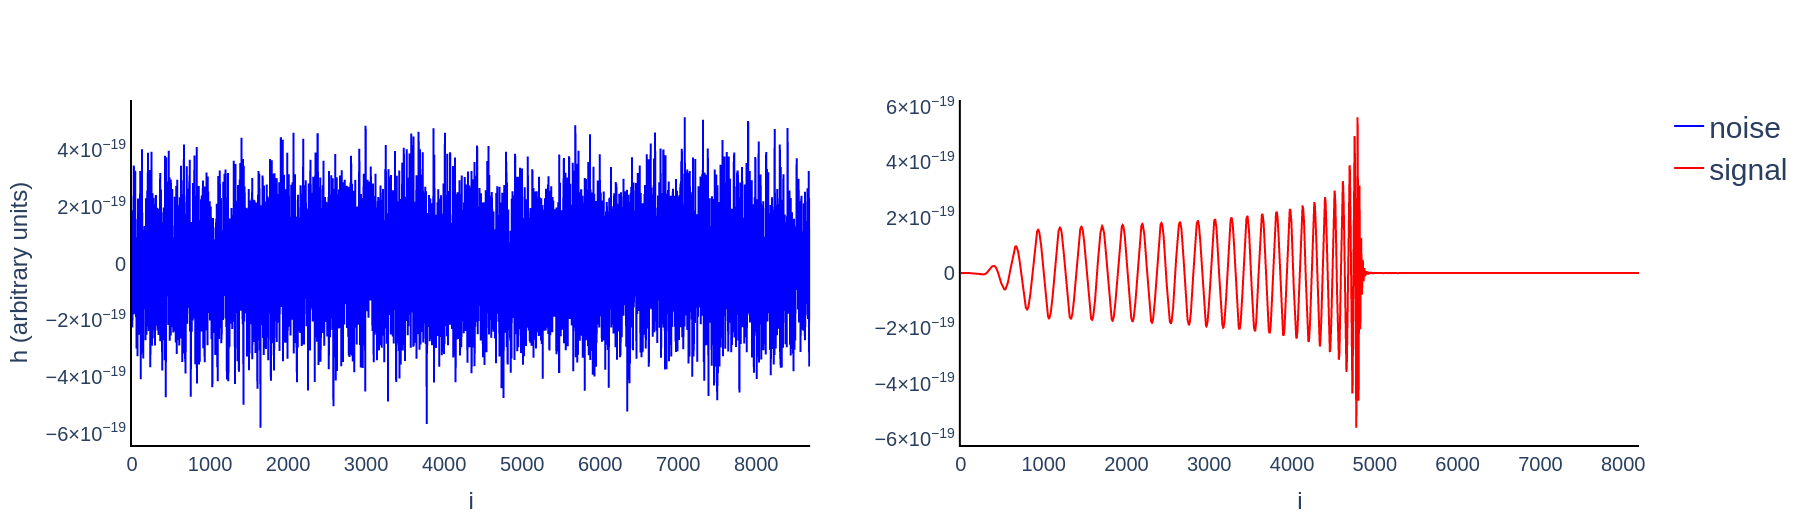
\includegraphics[width=\linewidth]{img/gw_and_noise}
	\\
}
\uncover<6->{
	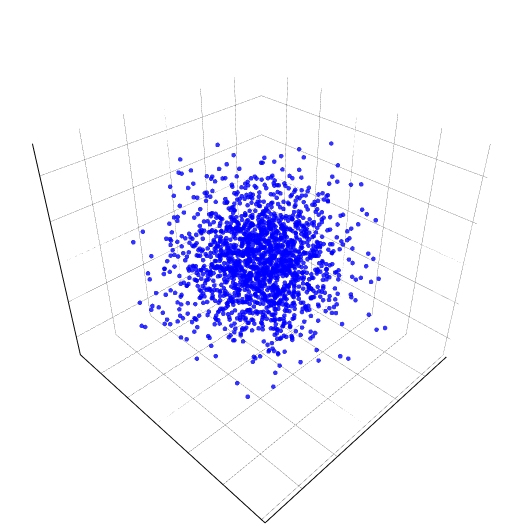
\includegraphics[width=0.35\linewidth]{img/noise_pointcloud}
}
	\hspace{0.1\linewidth}
\uncover<7->{
	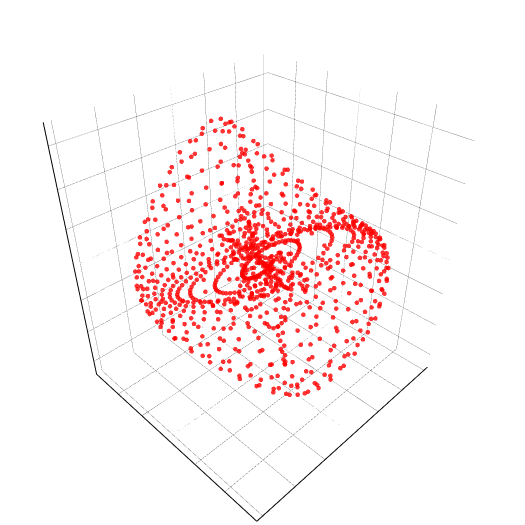
\includegraphics[width=0.35\linewidth]{img/gw_pointcloud}
}
\end{column}
\begin{column}{0.4\linewidth}
\uncover<2->{Taken's embedding:\\}
\begin{align*}
\uncover<3->{x(t) &= (x_1, x_2, \dots, x_i, x_{i+1}, \dots, x_n)}\\
\uncover<4->{t_i &= i \Delta t}\\~\\
\end{align*}

\begin{equation*}
\uncover<5->{
	x(t) \mapsto 
	\begin{pmatrix}
		x_{i} \\
		x_{i + \tau} \\
		\vdots \\
		x_{i + (d-1) \tau}
	\end{pmatrix}
}
\end{equation*}
\end{column}
\end{columns}
\end{frame}

\begin{frame}{Homology theory}
\uncover<+->{In simple terms, homology theory tries to connect the dots in a topological space together and figure out what shape they make\\}
\uncover<+->{To achieve this, homology theory uses \textit{Simplexes} and \textit{Simplical complexes}}
\begin{columns}
\begin{column}{0.4\linewidth}
\vskip .3cm
\centering
\uncover<+->{
	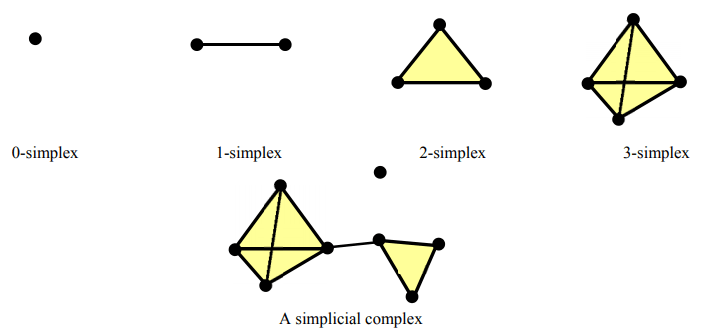
\includegraphics[width=\linewidth]{img/simplicial-complex}\\
	\textcolor{gray}{\fontsize{6.5}{10}\selectfont Image credit: \href{https://aaqr.org/articles/aaqr-18-08-oa-0315}{Zulkepli, et al.}}\\~\\
}
\uncover<4->{
	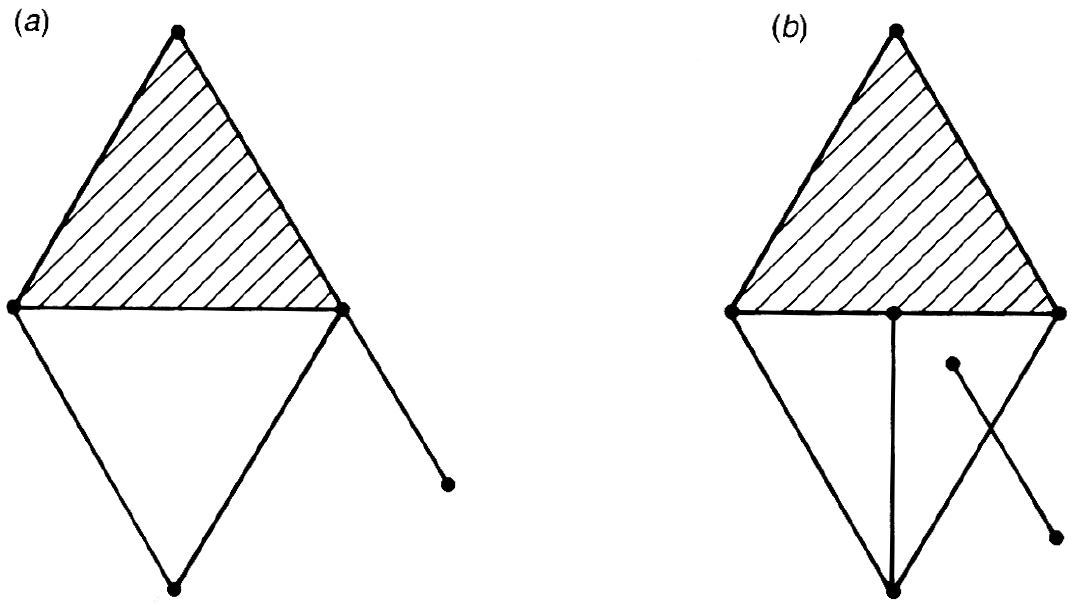
\includegraphics[width=.6\linewidth]{img/complex_not_complex}\\
	\textcolor{gray}{\fontsize{6.5}{10}\selectfont Image credit: \href{https://www.amazon.com/Geometry-Topology-Physics-Graduate-Student/dp/0750306068}{Nakahara}}\\~\\
}
\end{column}
\begin{column}{0.6\linewidth}
\begin{center}

\end{center}
\vskip -.5cm
\uncover<5->{Vietoris-Rips complex}
\begin{align*}
\uncover<6->{
	VR_s(\mathbb{X}) &=\\
	&\left\{\sigma^r = \langle p_0 \dots p_r\rangle ~\bigg\vert~ \forall p_i, p_j \in \sigma^r: ~l^2 (p_i, p_j) \leq s \right\}
}
\end{align*}
\centering
\uncover<7->{
	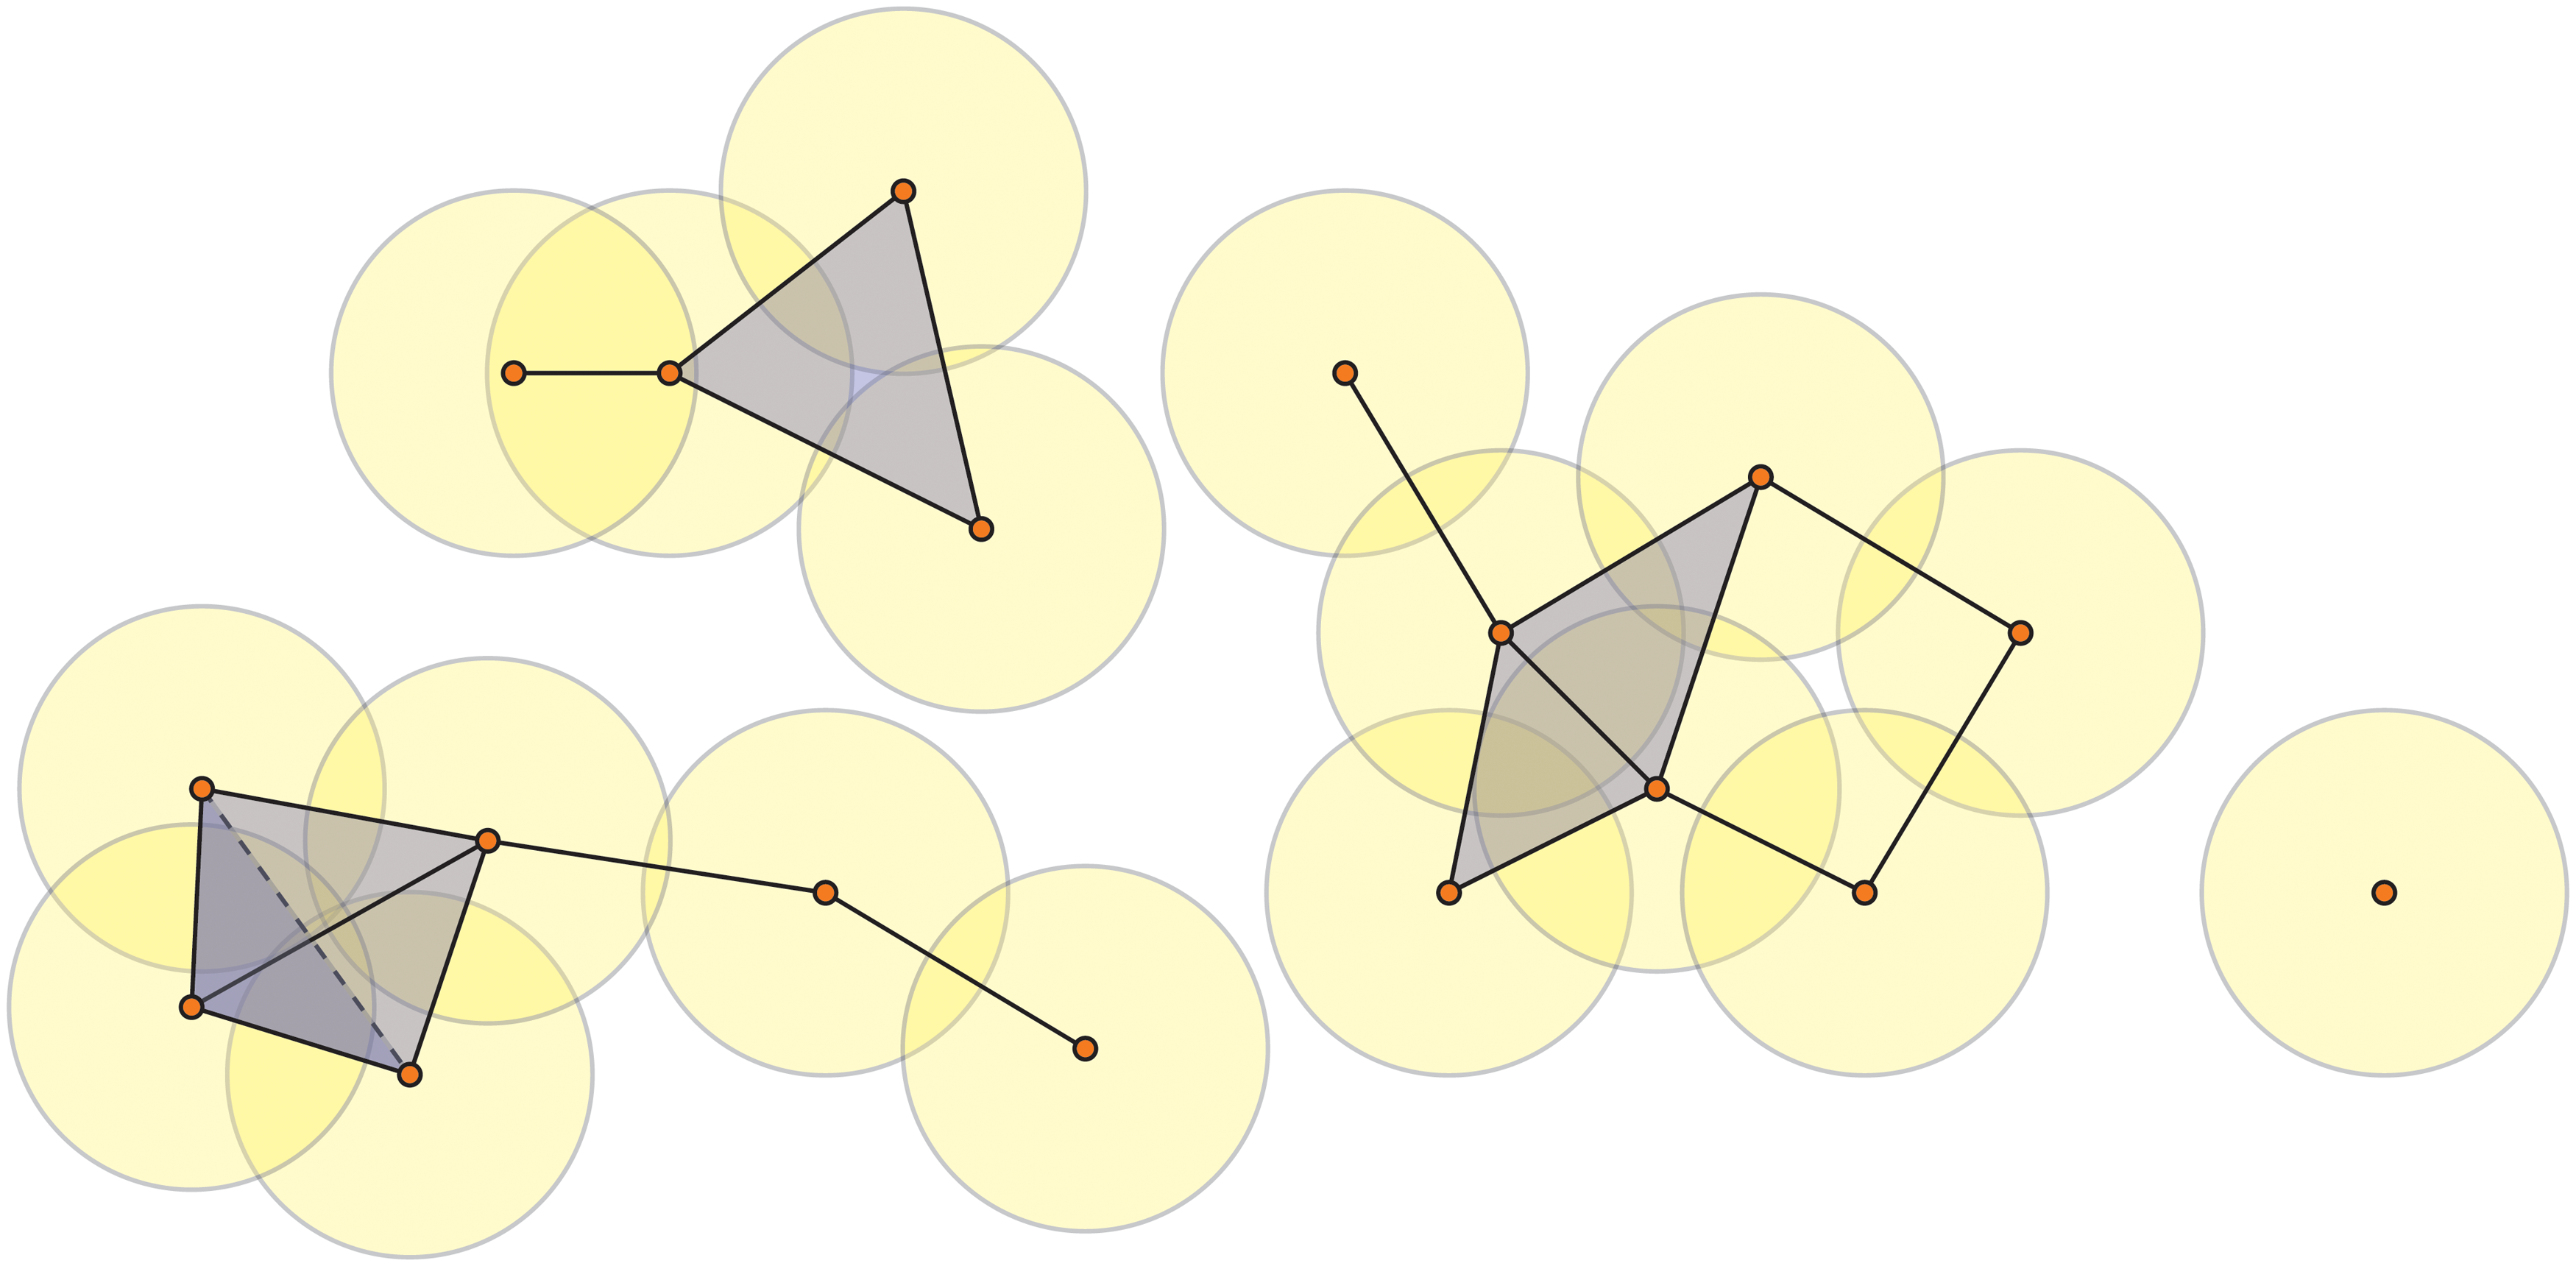
\includegraphics[width=0.75\linewidth]{img/VR_complex}\\
	\textcolor{gray}{\fontsize{6.5}{10}\selectfont Image credit: \href{https://journals.plos.org/plosone/article?id=10.1371/journal.pone.0126383}{Topaz, et al.}}
}
%\vspace*{0.5 cm}
\end{column}
\end{columns}

\end{frame}


\begin{frame}{Persistance homology}
\vskip .5cm
\centering
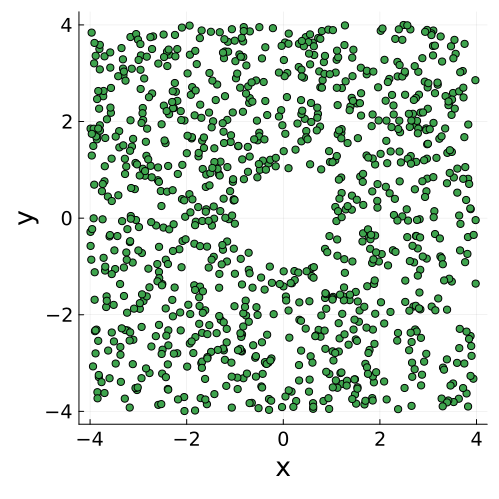
\includegraphics[width=.35\linewidth]{img/cut}
\hspace*{2cm}
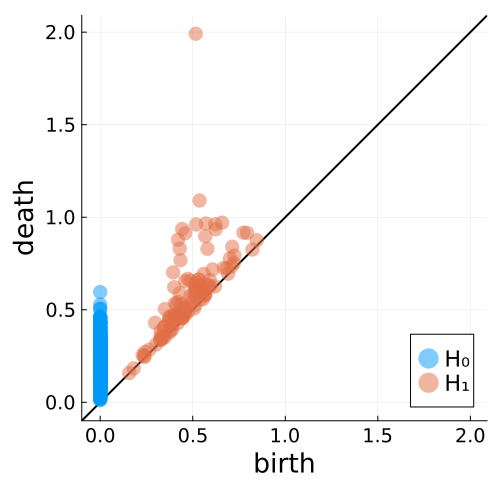
\includegraphics[width=.35\linewidth]{img/PD1}
\uncover<2->{$$\mathbb{X} = \{\mathbb{D}_0, \dots, \mathbb{D}_N\}$$}
\uncover<3->{$$\mathbb{D} = \{(b, d)~\vert~ 0 \leq b < d \in \mathbb{R} \}$$}
\end{frame}

\begin{frame}{Vectorizations and amplitudes}
\begin{columns}
\begin{column}{0.4\linewidth}
\begin{align*}
\uncover<+->{
	&\phi:~ \mathbb{X} \rightarrow \mathbb{V} \\~\\
}
\uncover<+->{
	&A:~ \mathbb{X} \rightarrow \mathbb{R}\\~\\
}
\uncover<+->{
	&A(s) = \vert\vert \phi(s) \vert\vert_p\\~\\
}
\uncover<+->{
	&\vert\vert x \vert\vert_p = (x_1^p + \dots + x_2^p)^{1/p}
}
\end{align*}
\end{column}
\begin{column}{0.6\linewidth}
\vskip -1cm
\centering
\uncover<5->{
	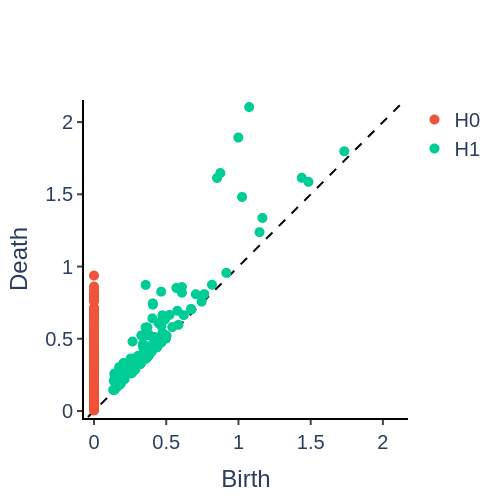
\includegraphics[height=0.35\textheight]{img/PD3.png}
}
\hspace{0.055\textheight}
\uncover<8->{
	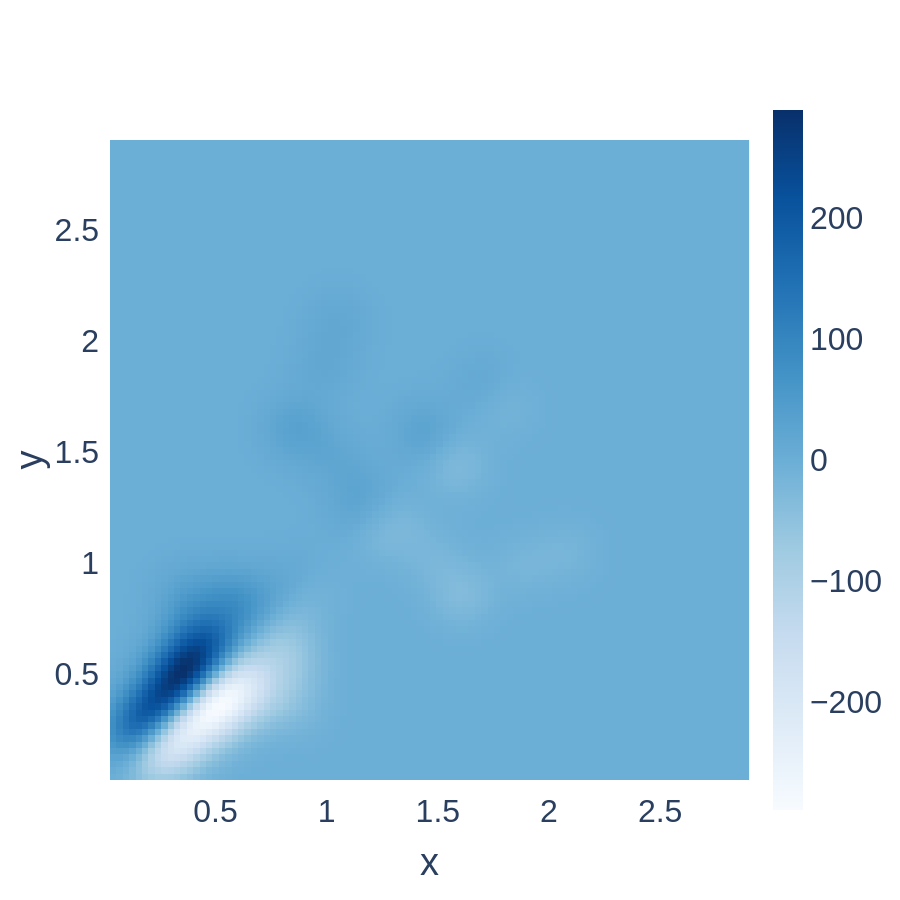
\includegraphics[height=0.35\textheight]{img/HK3.png}
}
\\
\uncover<6->{
	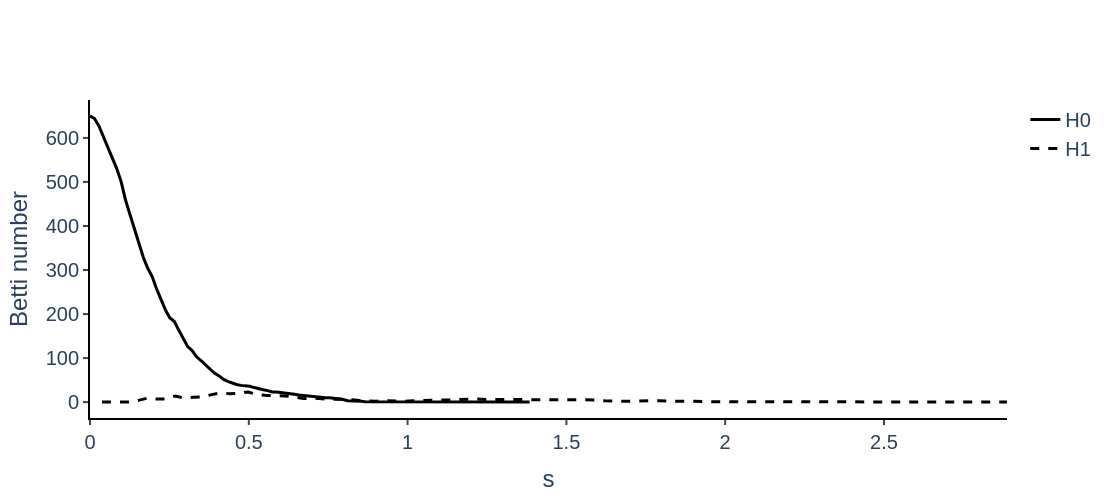
\includegraphics[height=0.35\textheight]{img/BC2.png}
}
\\
\uncover<7->{
	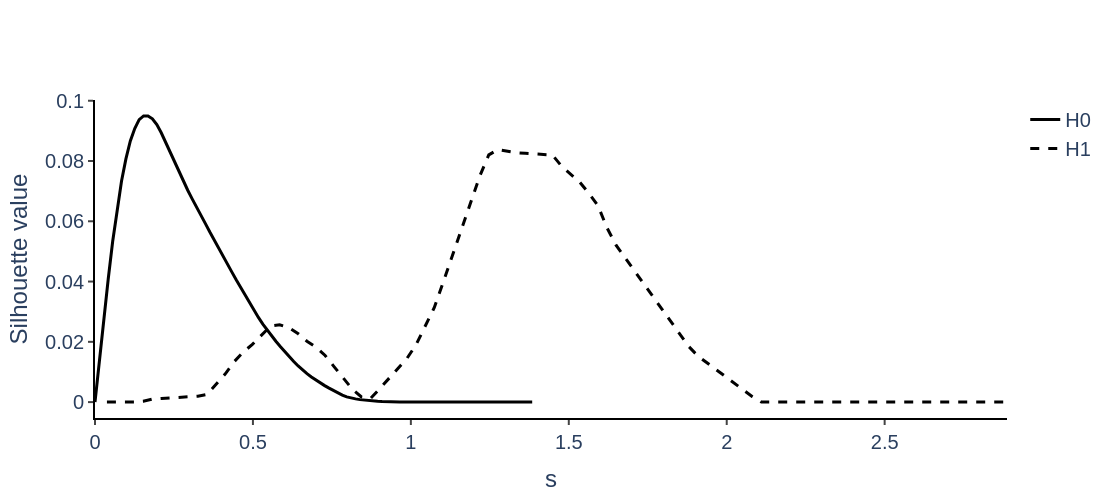
\includegraphics[height=0.35\textheight]{img/SIL2.png}
}
\end{column}
\end{columns}
\end{frame}

\begin{frame}{Recap}
	\uncover<+->{What we have by now:}
	\begin{itemize}[<+->]
		\item A model for primordial black hole binary mergers
		\item A way to simulate a stochastic background based on our model for different population statistics ($\sigma_{PBH}$)
		\item A data analysis method wich has a promise of being resiliant to noise
	\end{itemize}
	\vskip 1cm
	\uncover<+->{Now we are ready to build a data analysis model}\\
	\uncover<+->{We need to:}
	\begin{itemize}[<+->]
		\item Find topological features to detect a signal amidst different levels of noise
		\item Find topological features to discriminate between different values of $\sigma_{PBH}$
		\item A classification method to classify signals with different values of $\sigma_{PBH}$
	\end{itemize}
\end{frame}